\chapter{大气强迫降尺度}\label{大气强迫降尺度}
%\addcontentsline{toc}{chapter}{大气强迫降尺度}
%\begin{大气强迫降尺度}
\begin{mymdframed}{代码}
本章节对应代码包含于\texttt{MOD\_ForcingDownscaling.F90}。
\end{mymdframed}

本模块通过地形调整和机器学习降尺度算法将模式网格(Element)上的大气强迫场降尺度到次网格(Patch)上。
针对的大气状态变量为大气温度($T_{a}$),近地面气压($P_{a}$),大气比湿($q_{a}$),大气风速($u_{a}$),近地面下行长波辐射($L↓$),近地面下行短波辐射($S↓$)和降水($p$),并相应调整了位温($\theta_{a}$)和大气密度($\rho_{a}$)。

\section{大气温度降尺度}
大气温度由地形偏差和温度递减率(${\Gamma}_{t}$)调整:
\begin{equation}\label{T_atm}
\hat{T_{a}}=T_{a}-{\Gamma}_{t} \left(\hat{z}-z\right)
\end{equation}
其中,
${\Gamma}_{t}=0.006$(每上升1000 m下降6度)。
$z$, $\hat{z}$分别为模式网格和次网格上的海拔高度,
$T_{a}$, $\hat{T_{a}}$分别为模式网格和次网格上的温度。

\section{近地面气压降尺度}
近地面气压由地形偏差和大气温度调整~\citep{Cosgrove2003}。

基于流体静力方程和理想气体假设,可推导:
\begin{equation}
\partial z=-\frac{RT_{a}}{g}\frac{\partial P_{a}}{P_{a}}
\end{equation}
其中,$z$为高度,$R$为干空气常数,$g$为重力加速度。

如采用均温假设,可推导:
\begin{equation}
\hat{P_{a}}=P_{a} \exp{\left(-\frac{\hat{z}-z}{\bar{z}}\right)}
\end{equation}
其中,
$\bar{z}$为地形调整前后平均温度对应的标高,计算方式为$\bar{z}=\frac{R}{g} \frac{\hat{T_{a}}+T_{a}}{2}$,  
$P_{a}$, $\hat{P_{a}}$分别为模式网格和次网格上的气压。

如采用温度线性递减假设(即${\Gamma}_{t}=0.006$),可推导:
\begin{equation}
\hat{P_{a}}=P_{a} \frac{\hat{T_{a}}}{T_{a}}^\frac{g}{R\Gamma_{t}}
\end{equation}

\section{位温降尺度}
对大气温度和近地面气压降尺度后,更新次网格上的位温:

位温定义为:
\begin{equation}\label{eq:位温定义}
\theta_{a}=T_{a} \left(\frac{P_0}{P_{a}}\right)^\frac{R}{C_{p}}
\end{equation}

近地面气压为:
\begin{equation}\label{eq:近地面气压}
{P_{a}}=P_{0} e^{-\frac{z_{a}}{\bar{H}}}
\end{equation}
%
代入~\eqref{eq:位温定义},可得:
\begin{equation}\label{eq:theta_atm}
\theta_{a}=T_{a} e^{\frac{z_{a}}{\bar{H}} \frac{R}{C_{p}}}
\end{equation}

根据~\eqref{eq:theta_atm},位温可由大气温度偏差调整为:
\begin{equation}
\hat{\theta_{a}}=\theta_{a}+\left(\hat{T_{a}}-T_{a}\right) e^{\frac{z_{a}}{\bar{H}} \frac{R}{C_{p}}}
\end{equation}
其中,
$P_{0}$为标准大气压,
$\frac{R}{C_{p}}$为干绝热指数,约为0.286,
$z_{a}$为参考高度。
$\theta_{a}$, $\hat{\theta_{a}}$分别为模式网格和次网格上的位温。

\section{比湿降尺度}
大气比湿由估计的饱和比湿比例来调整:
\begin{equation}
\hat{q_{a}}=q_{a} \frac{\hat{q_{sat}^T}}{q_{sat}^T} 
\end{equation}
其中,模式网格和次网格上的饱和比湿通过降尺度前后的大气温度计算(附录~\ref{饱和水汽压(比湿)及其随温度的变化})。注意该方案的假设为降尺度前后满足相对湿度守恒。

\section{大气密度降尺度}
调整大气温度,近地面气压和大气比湿后,更新次网格上的大气密度:
\begin{equation}
\rho_{a}=\frac{P_{a}-(1-\phi)A}{R T_{a}}
\end{equation}
其中,$\phi$为水蒸气与干空气的分子量比值,为0.62197。$A=\frac{q_{a} P_{a}}{\phi +(1-\phi)q_{a}}$。

\section{大气风速降尺度}\label{大气风速降尺度}
大气风速由地形因子调整~\citep{liston2006Meteorological},计算为:
\begin{equation}
\hat{u_{a}}=\left(1+\zeta_{s}\omega_{s}+\zeta_{c}\omega_{c}\right)u_{a}
\end{equation}
其中,$\omega_{s}$为沿风向上地形的坡度,计算为:
\begin{equation}
\omega_{s}=\alpha \cos{\left(\theta-\beta\right)}
\end{equation}
其中,$\theta$为风向。$\alpha$和$\beta$为地形的坡度和坡向,分别计算为:
\begin{equation}
\alpha=\arctan \sqrt{\frac{\partial z}{\partial x}+\frac{\partial z}{\partial y}}
\end{equation}
%
\begin{equation}
\beta=\begin{cases}
    \frac{3\pi}{2}-\arctan \frac{\frac{\partial z}{\partial y}}{\frac{\partial z}{\partial x}} & \text{当}\quad \frac{\partial z}{\partial x}>0 \\
    \frac{\pi}{2}-\arctan \frac{\frac{\partial z}{\partial y}}{\frac{\partial z}{\partial x}} & \text{当}\quad \frac{\partial z}{\partial x}<0 \\
    0 & \text{当}\quad \frac{\partial z}{\partial x}=0\quad \text{且}\quad \frac{\partial z}{\partial y}<0 \\
    \pi & \text{当}\quad \frac{\partial z}{\partial x}=0\quad \text{且}\quad \frac{\partial z}{\partial y}>0 
\end{cases}
\end{equation}
$\omega_{c}$为地形的曲率,计算为:
\begin{equation}
   \begin{split}
    \omega_{c}=&\frac{1}{4}\left[\frac{z-1/2\left(z_{W}+z_{E}\right)}{2\eta}+\frac{z-1/2\left(z_{S}+z_{N}\right)}{2\eta}\right. \\
    & \left.+\frac{z-1/2\left(z_{SW}+z_{NE}\right)}{2\sqrt{2}\eta}+\frac{z-1/2\left(z_{NW}+z_{SE}\right)}{2\sqrt{2}\eta}\right]
   \end{split}
\end{equation}
其中,$z_{[W,E,S,N,SW,NE,NW,SE]}$分别代表临近的8个网格的海拔。$\eta$是网格的长度。坡度与曲率均被归一化至$[-0.5,0.5]$。$\zeta_{s}$和$\zeta_{c}$为根据地形的坡度和曲率调整风速的比例,两者求和为1。在CoLM中设定为$\zeta_{s}=0.58$,$\zeta_{c}=0.42$。为保证风速降尺度后处于合理的数值范围,其调整的权重($1+\zeta_{s}\omega_{s}+\zeta_{c}\omega_{c}$)被限制在$[0.5,1.5]$。

\section{近地面下行长波辐射降尺度}
近地面下行长波辐射调整方案分为两种:

第一种方案~\citep{fiddes2014toposcale} 为:

晴朗天空发射率由水汽压和大气温度计算获得~\citep{konzelmann1994parameterization}:
\begin{equation}\label{eq:varepsilon_c}
\varepsilon_{c}=0.23+0.43 \left(\frac{e^{T}}{T_{a}}\right)^\frac{1}{5.7}
\end{equation}
其中,$e^{T}$为水汽压,由饱和水汽压和比湿计算而得$e^{T}= \frac{q_{a} e_{sat}^{T}}{100}$,饱和水汽压由大气温度计算获得(附录~\ref{饱和水汽压(比湿)及其随温度的变化})。将模式网格和次网格的大气温度代入公式~\eqref{eq:varepsilon_c},得到对应网格的晴空发射率$\varepsilon_c$和$\hat{\varepsilon_{c}}$。

全空发射率由斯蒂芬-玻尔兹曼公式计算而得: 
\begin{equation}
\varepsilon_{a}=\frac{L↓}{\sigma T_{a}^4}
\end{equation}
其中,$\sigma$为斯蒂芬-玻尔兹曼常数。则多云天空发射率为$\varepsilon_{cl}=\varepsilon_{a}-\varepsilon_{c}$。

近地面入射长波辐射调整为:
\begin{equation}
\hat{L}↓=\left(\varepsilon_{cl}+\varepsilon_{c}\right) \sigma \hat{T_{a}}^4
\end{equation}

第二种方案~\citep{Tricht2016}假设近地面入射长波辐射与海拔高度呈现线性反比的关系。计算方案为:

对于冰川覆盖类型:
\begin{equation}
\hat{L}↓=L↓-\Gamma_{l} \left(\hat{z}-z\right)       
\end{equation}

对于其他覆盖类型:
\begin{equation}
\hat{L}↓=L↓-\frac{4 L↓}{\bar{T_{a}}} \Gamma_{t} \left(\hat{z}-z\right)      
\end{equation}
其中,$\Gamma_{l}=0.032$,$L↓$, $\hat{L↓}$分别为模式网格和次网格上的入射长波辐射。

为保证对长波辐射降尺度后数值与原始数值不会相差较大,因此将其数值控制在原始数值的0.5--1.5倍之间。注意,为保证降尺度前后的总长波辐射量守恒,将降尺度前后长波辐射总量的比值作为权重系数调整次网格上的长波辐射。

\section{近地面下行短波辐射降尺度}
短波辐射降尺度由四个步骤组成:将入射短波辐射分解成漫射与直射辐射;订正直射辐射;订正漫射辐射;基于订正后的直射和漫射辐射计算反射辐射。

漫射辐射占总辐射的比例($k$)由基于大气透明度($k_{t}$)的回归方程得出~\citep{ruizarias2010}:
\begin{equation}
k=a_{0}+a_{1} \times \exp \big(- \exp \left( a_{2}+a_{3} \times k_{t} \right) \big)
\end{equation}
其中,回归系数来自于对欧洲与美国21个逐小时站点数据的拟合,$a_{0}$、$a_{1}$、$a_{2}$、$a_{3}$分别为$0.952$,$-1.041$,$2.3$,$-4.702$。大气透明度定义为到达地面的入射短波辐射($I_{G}$)与大气层顶入射短波辐射($I_{0}$)的比值。大气层顶的入射短波辐射($I_{0}$)定义为:
\begin{equation}
I_{0}=S \times \cos{\left(\theta_{z}\right)} \times R^{2}
\end{equation}
其中,太阳常数$S=1370$ \unit{W.m^{2}},$\theta_{z}$为太阳天顶角。$R$为日地距离,可由年积日(day of year,$DOY$)计算得~\citep{eva1998}:
\begin{equation}
R=1-0.01672 \times \cos{\big( 0.9856 \times \left(DOY-4 \right)\big)}
\end{equation}
由所得漫射比例($k$),可将入射短波辐射($S\downarrow$)分解为漫射辐射($S_{d}\downarrow$)与直射辐射($S_{b}\downarrow$)(图~\ref{fig:短波直射调整图}(A))。

直射辐射由三个因子订正,消光系数(图~\ref{fig:短波直射调整图}(B)),局地照明角(图~\ref{fig:短波直射调整图}(C))和遮蔽系数(图~\ref{fig:遮蔽因子示意图})。

消光系数($k_{e}$)由大气透明度($k_{t}$)~\citep{gupta2016}计算获得:
\begin{equation}
k_{e}=\frac{\ln{\left(k_{t}\right)}}{P_{a}}
\end{equation}
基于Beer-Lambert定律,降尺度后,直射辐射随光程变化的调整因子计算为:
\begin{equation}
\hat{\psi}=\exp{\left[ -k_{e} \times \left(\hat{P_{a}}-P_{a} \right) \right]} 
\end{equation}
其中,$\hat{P_{a}}$为降尺度后的近地面气压。

局地照明角($\theta_{i}$)指直射辐射与地形平面法线的夹角,计算为:
\begin{equation}
\cos{\theta_{i}}=\cos{\theta_{z}}\cos{\beta}+\sin{\theta_{z}}\sin{\beta}\cos{\left(\theta_{a}-\alpha\right)}
\end{equation}
其中,$\theta_{a}$是太阳方位角。$\alpha$和$\beta$是地形的坡向和坡度(计算方式见~\ref{大气风速降尺度})。

{
\begin{figure}[htbp]
\centering
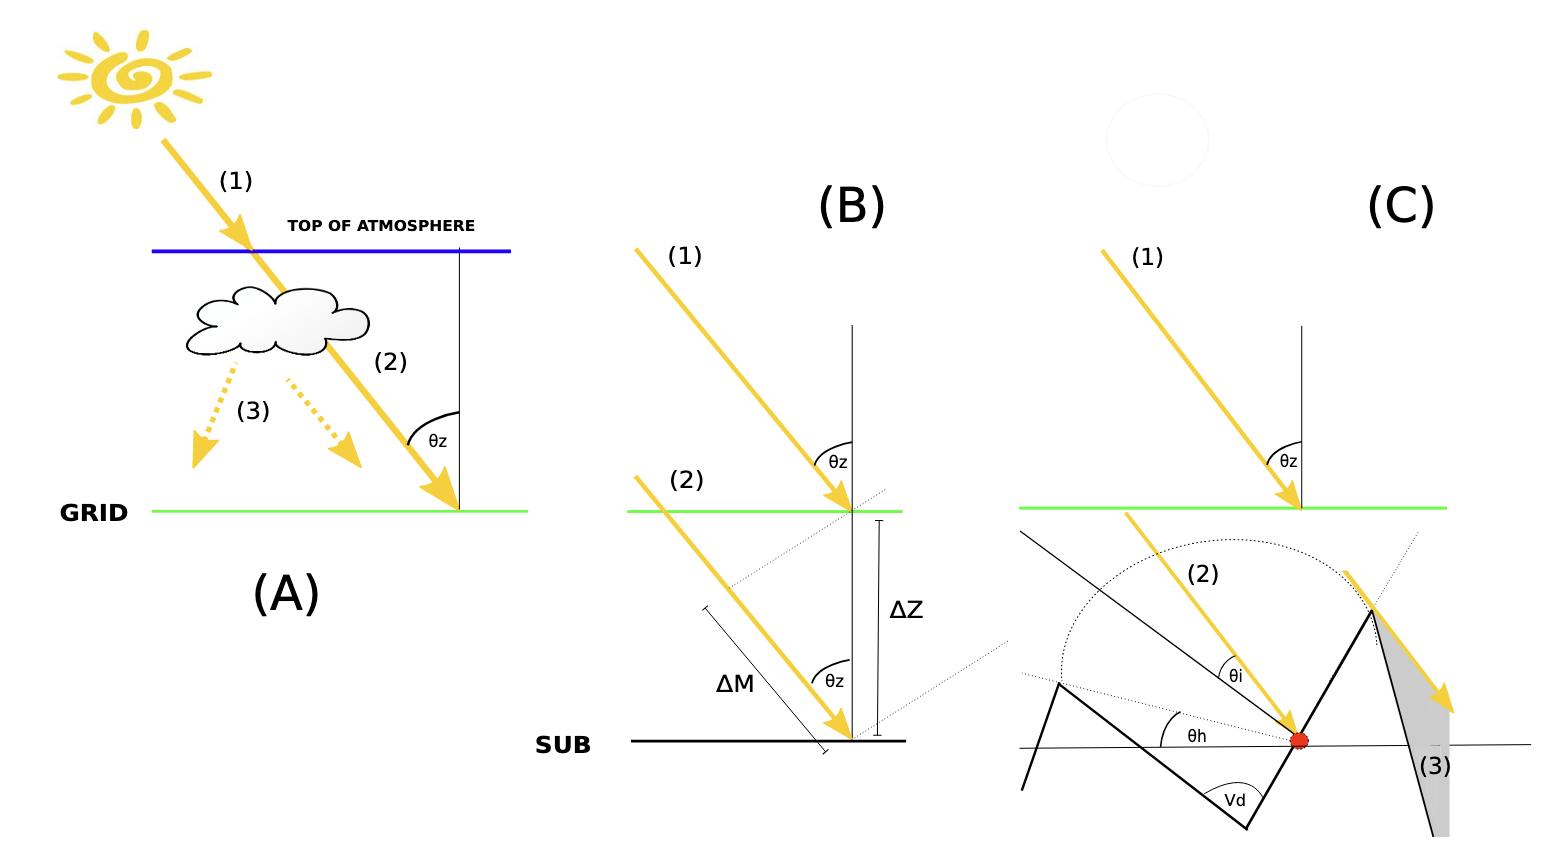
\includegraphics[width=0.97\textwidth]{Figures/尺度转换/短波直射调整图.png}
\caption[短波直射调整示意图]{短波直射调整示意图。(A) 短波基于大气透明度分解为直射(1)和漫射(3)。(B) 由于地形变化($\Delta Z$)导致光程的变化($\Delta M$),模式网格上的直射(1)通过消光系数订正为次网格上的直射(2)。(C) 由于地形的差异,直射辐射经过照明角调整至与地形垂直的法线方向。图片摘自~\citep{fiddes2014toposcale}}
\label{fig:短波直射调整图}
\end{figure}
}

遮蔽系数用于判断格点是否处于地形遮挡而形成的投射阴影下。采用WRF中对遮蔽系数的计算方式,流程如下:
\begin{enumerate}
    \item 根据太阳方位角确定太阳相对于地形的位置(北、东、南、西侧),从而确定搜索地形的方向。具体搜索方向见表~\ref{tab:遮蔽因子搜索方向}。
    \item 沿着搜索方向逐网格搜索,计算投影在太阳方位角方向的坐标位置。以太阳处于地形北部为例(见图~\ref{fig:遮蔽因子示意图}),假设沿y轴正半轴搜索到第$j$个网格,则投影在方位角方向的坐标为$(ii,j)=(j \tan\theta_{a},j)$,其中$i \leqslant ii \leqslant i+1$。
    \item 计算$(ii,j)$相对于$(0,0)$坐标的长度,即$l_{\left(ii,j\right)}=\eta\sqrt{ii^{2}+j^{2}}$。同时通过加权平均的方式计算$(ii,j)$位置的海拔,即$z_{\left(ii,j\right)}=\left(ii-i\right)z_{\left(i+1,j\right)}+\left(1+i-ii\right)z_{\left(i,j\right)}$。
    \item 计算沿太阳方位角方向的地形坡度角$\theta_{s}=\arctan\left(z_{\left(ii,j\right)}/l_{\left(ii,j\right)}\right)$。
    \item 最后通过地形坡度角与太阳高度角的位置判断该地区是否被遮蔽。如果当前搜索网格没有遮蔽,则会继续搜索,直到到达搜索半径($d$)。
    \begin{equation}
    \delta=\begin{cases}
        0 & \text{当}\ \theta_{z} \leqslant \theta_{s} \\
        1 & \text{当}\ \theta_{z} > \theta_{s} \\ 
    \end{cases}
    \end{equation}
\end{enumerate}

由于该方案针对每个网格均需搜索$d$次,在高分辨率模拟中计算复杂度过高,只适用于粗分辨率的模拟。CoLM基于~\citet{zhang3d2022}额外提供查找表的简化方案。即将$[0,360]$的方位角进行240等分,针对原始高程数据的每个网格,分别计算240种太阳方位角对应的遮蔽系数。在模式中,只需判断方位角的位置,即可获得对应网格点的遮蔽系数值。

\begin{table}[htbp]
    \centering
    \caption{遮蔽系数搜索方向}
    \label{tab:遮蔽因子搜索方向}
    \begin{threeparttable}
    \begin{tabular}{ccc}
    \toprule
    太阳相对于地形位置 & 搜索方向 & 太阳方位角范围  \\  \midrule
    北 & y轴正半轴 & $1.75\pi \leqslant \theta_{a} \leqslant 2\pi$ \text{或} $0 \leqslant \theta_{a} < 0.25\pi$   \\
    东 & x轴正半轴 & $0.25\pi \leqslant \theta_{a} < 0.75\pi$ \\
    南 & y轴负半轴 & $0.75\pi \leqslant \theta_{a} < 1.25\pi$ \\
    西 & x轴负半轴 & $1.25\pi \leqslant \theta_{a} < 1.75\pi$ \\
    \bottomrule
    \end{tabular}
    \end{threeparttable}
\end{table}

{
\begin{figure}[htbp]
\centering
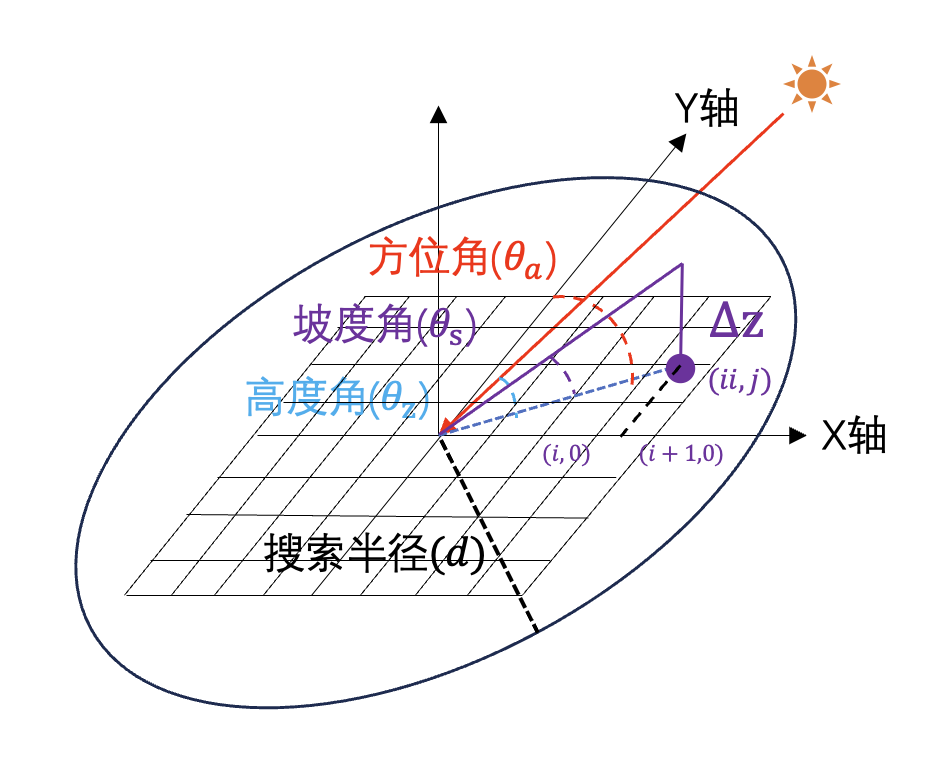
\includegraphics[width=0.8\textwidth]{Figures/尺度转换/遮蔽因子示意图.png}
\caption{遮蔽因子示意图}
\label{fig:遮蔽因子示意图}
\end{figure}
}

则直射辐射降尺度计算为:
\begin{equation}
\hat{S_{b}\downarrow}=S_{b}\downarrow \times \hat{\psi} \times \cos{\theta_{i}} \times \delta 
\end{equation}

降尺度后,漫射辐射由于地形遮挡,只能接收部分天空发射的漫射辐射,用天空可视因子$F_{v}$对漫射辐射订正:
\begin{equation}
\hat{S_{d}\downarrow}=S_{d}\downarrow F_{v}
\end{equation}
其中,$F_{v}$采用~\citet{dozier1990}的方案:
\begin{equation}
V_{d}=\frac{1}{2\pi} \int_{0}^{2\pi} [\cos{\alpha}\sin^2{\zeta}+\sin{\alpha}\cos{\left(\theta_{a}-\beta\right)}\left(\zeta-\sin{\zeta}\cos{\zeta}\right)]d\theta_{a}
\end{equation}
其中,$\zeta$代表搜索半径内最大地形与垂直线的夹角,与太阳高度角($\theta_{a}$)相关。

反射辐射由降尺度后的直射辐射($S_{b}\downarrow$)和散射辐射($S_{d}\downarrow$)计算得到~\citep{tao2018}:
\begin{equation}
S_{f}=A F_{t} [\hat{S_{b}\downarrow}+\left(1-F_{v}\right)\hat{S_{d}\downarrow}]
\end{equation}
其中,$A$是次网格上一步更新的地表反照率,$F_{t}$为地形结构因子,计算为:
\begin{equation}
F_{t}=0.5 \times \left(1+\cos{\beta}\right)-V_{d}
\end{equation}

最后,降尺度后的短波辐射是降尺度后的直射辐射,漫射辐射和反射辐射之和:
\begin{equation}
\hat{S_{d}\downarrow}=\hat{S_{b}\downarrow}+\hat{S_{d}\downarrow}+\hat{S_{f}\downarrow}
\end{equation}

\section{降水降尺度}
降水提供两种地形降尺度方案和一种机器学习降尺度方案:

第一种方案~\citep{Tesfa2020}为:
\begin{equation}
\hat{p}=p \left({1+\frac{\hat{z}-z}{\hat{z_{max}}}}\right)
\end{equation}
其中,$\hat{z_{max}}$为次网格上最大海拔高度,
$p$、$\hat{p}$分别为模式网格和次网格上的降水。

第二种方案~\citep{liston2006Meteorological}为:
\begin{equation}
\hat{p}=p \left(1+\frac{2 \times 0.00027 \times \left(\hat{z}-z\right)}{1- 0.00027 \times \left(\hat{z}-z\right)}\right)
\end{equation}

第三种方案基于~\citep{mei2020}调整:

基于机器学习的降水降尺度需要构建分类模型和预报模型。分类模型用于提供是否降水的判断,预报模型用于降水量的估计。其训练过程如下:

\begin{enumerate}
    \item 生成模式网格下的降水掩码$p_{m}$(设定阈值为$0.01$ \unit{mm.h^{-1}},高于阈值为$1$,低于阈值为$0$)。
    \item 选定模型的预报因子$\Omega$(见表~\ref{tab:降水降尺度模型的输入特征})。
    \item 基于粗分辨率数据拟合$p_{m}=G_{c}\left(\Omega\right)$关系。$G_{c}$为随机森林分类模型。
    \item 基于粗分辨率数据拟合$p[p_{m}=1]=G_{r}\left(\Omega[p_{m}=1]\right)$关系。$G_{r}$为随机森林回归模型。
    \item 基于上述地形降尺度方案对$u_{a}$、$d_{a}$、$T_{a}$、$q_{a}$、$P_{a}$、$L\downarrow$和$S\downarrow$降尺度,得到的细分辨率特征。则降尺度后的降水$\hat{p}=G_{c}\left(\hat{\Omega}\right) \cdot G_{r}\left(\hat{\Omega}\right)$。
\end{enumerate}

随机森林模型~\citep{rf2001}是基于随机决策树的集成学习算法。参数基于optuna库来优化,其参数优化范围见~\ref{tab:随机森林模型参数优化范围}。注意,随机森林模型的选择是基于ERA5大气强迫场降尺度的前期实验,发现其优于其他主流机器学习模型。

值的注意的是,当前CoLM仅支持耦合离线训练的机器学习模型,即针对每次具体任务(特定区域、特定大气强迫)均需重新训练机器学习模型。然后通过MPI通讯的方式耦合CoLM和训练好的离线模型(见~\ref{CoLM和机器学习模型在线耦合})。

\begin{table}[htbp]
    \centering
    \caption{降水降尺度模型的输入特征}
    \label{tab:降水降尺度模型的输入特征}
    \begin{threeparttable}
    \begin{tabular}{ccc}
    \toprule
    特征变量               & 变量名           & 单位           \\  \midrule
    位于参考高度的风速 & $u_{a}$     & \unit{m.s^{-1}}   \\
    位于参考高度的露点温度 & $d_{a}$ & \unit{K} \\
    位于参考高度的大气温度 & $T_{a}$     & \unit{K}            \\
    位于参考高度的大气比湿 & $q_{a}$     & \unit{kg.kg^{-1}} \\
    近地面气压                & $P_{a}$     & Pa           \\
    近地面下行长波辐射            & $L\downarrow$ & \unit{W.m^{-2}}   \\
    近地面下行短波辐射            & $S\downarrow$ & \unit{W.m^{-2}}   \\
    海拔高度 & $z$ & \unit{m} \\
    年积日 & $DOY$ & [-] \\
    经度 & $lat$ & \unit{\deg} \\
    纬度 & $lon$ & \unit{\deg} \\
    \bottomrule
    \end{tabular}
    \begin{tablenotes}
    \footnotesize
    \item[注:] 应结合具体大气强迫资料与选定区域来筛选特征变量。
    \end{tablenotes}
    \end{threeparttable}
\end{table}

\begin{table}[htbp]
    \centering
    \caption{随机森林模型参数优化范围}
    \label{tab:随机森林模型参数优化范围}
    \begin{threeparttable}
    \begin{tabular}{ccc}
    \toprule
    参数 & 变量名 & 取值 \\ \midrule
    树的个数 & \texttt{n\_estimators} & [50, 100, 150, 200] \\
    树的最大深度 & \texttt{max\_depth} & [1, 10] \\
    叶节点上最少样本量 & \texttt{min\_samples\_leaf} & [5, 10, 15, 20, 25, 30] \\
    \bottomrule
    \end{tabular}
    \begin{tablenotes}
    \footnotesize
    \item[注:] 参数变量名来自sklearn库。参数需结合具体大气强迫资料来调整,也可使用FLAML自动机器学习库优化。
    \end{tablenotes}
    \end{threeparttable}
\end{table}


\section{CoLM和机器学习模型的耦合}\label{CoLM和机器学习模型在线耦合}
CoLM与机器学习模型的在线耦合,本质是解决Fortran与Python的异构问题。在当前CoLM中实现的方案流程如下:
\begin{enumerate}
    \item 在总MPI空间中,将CoLM和Python进程分别染色成两个子空间。此时CoLM内部的spmd并行启动直接用子空间传参,并不另外额外进行MPI$\_$init,这与CoLM与CAS-ESM或CWRF的耦合是一致的。此外在Python中不设计内部分组等细分,仅需染色区分CoLM组即可。
    \item 以耦合降水降尺度模型为例,操作如下:
    
    a. 找到对应计算的子程序,厘清输入输出;
    
    b. 在Fortran中准备好机器学习模型中所需的输入特征; 
    
    c. 将输入变量打包(或不打包,皆可)通过mpi$\_$send程序传递给Python进程,此时mpi$\_$send需要在全局通讯空间进行,索引到Python的进程空间中。索引方式可以多种多样,只需要指向正确的Python进程即可。Python部分需要做的事情相对简单类似于若干台长期开机的服务器,做好接收-计算-返回三个环节即可。
    \item 在整个环节中,需要注意的额外问题:
    
    a. 总体计算效率,尤其Python中的算法计算效率需要重点关注,采用负载均衡的设计使得Python进程可以以合理的效率处理好计算任务。
    
    b. 确保计算寻址正确,在Python的MPI传递和接收中需要探明传入来源,确保计算返回到正确的Fortran进程中。
    
    c. 做好验证工作,当前框架初建尚未在足够多的场景中进行测试,因此在实装中需要先用单点测试结果正确性,同时强烈建议先在Python中重写原来需要替换的算法,原装算法验证结果无误之后再实现新算法的应用。
\end{enumerate}

